\documentclass[12pt]{article}

\usepackage{xspace}
\usepackage{lineno}
\usepackage{setspace}
\usepackage{graphicx}
\usepackage{subfigure}
\usepackage{float}
\usepackage{color}
\usepackage{caption}
\usepackage[margin=1in]{geometry}
\usepackage{natbib}
\usepackage{amsmath}
\usepackage{hyperref}


%\setlength{\marginparwidth}{1in}
\let\oldmarginpar\marginpar
\renewcommand\marginpar[1]{\-\oldmarginpar[\raggedleft\tiny #1]%
{\raggedright\tiny #1}}

\begin{document}
\doublespacing
\linenumbers

\newcommand{\kluyveri}{\textit{L. kluyveri}\xspace}
\newcommand{\dubl}{\textit{C. dubliniensis}\xspace}
\newcommand{\gossypii}{\textit{E. gossypii}\xspace}
\newcommand{\ROC}{ROC SEMPPR\xspace}
\newcommand{\GC}{GC content\xspace}
\newcommand{\DM}{\ensuremath{{\Delta M}}\xspace}
\newcommand{\DE}{\ensuremath{{\Delta \eta}}\xspace}

\newcommand{\beginsupplement}{%
        \setcounter{table}{0}
        \renewcommand{\thetable}{S\arabic{table}}%
        \setcounter{figure}{0}
        \renewcommand{\thefigure}{S\arabic{figure}}%
     }

\noindent RH: LANDERER ET AL.--- Intragenomic variation in codon usage
% put in your own RH (running head)
% for POVs the RH is always POINT OF VIEW
\bigskip
\medskip
\begin{center}

% Insert your title:
\noindent{\Large \bf Fitness consequences of mismatched codon usage}
\bigskip

% We don't use a special title page; the author information is entered
% like any other text.

% FOOTNOTES: We don't allow them in the manuscript, except in
% tables. Don't include any footnotes in the text.


\noindent{C\textsc{EDRIC} ~{L\textsc{ANDERER}}$^{1,2,*}$,
R\textsc{USSELL} {Z\textsc{ARETZKI}}$^{3}$,
\textsc{AND}
M\textsc{ICHAEL} A.~{G\textsc{ILCHRIST}}$^{1,2}$}

\end{center}

\vfill

{\small
\noindent$^{1}$Department of Ecology \& Evolutionary Biology, University of Tennessee, Knoxville, TN 37996-1610\\
\noindent$^{2}$National Institute for Mathematical and Biological Synthesis, Knoxville, TN 37996-3410\\
\noindent$^{3}$Department of Business Analytics \& Statistics, Knoxville, TN ~ 37996-0532 \\
\noindent$^{*}$Corresponding author. E-mail:~cedric.landerer@gmail.com
}

\vfill
\centerline{Version dated: \today}
\vfill
\newpage

\begin{abstract}
Codon usage has been used as a measure for adaptation of genes to their genomic environment for decades. 
The introgression of genes from one genomic environment to another may cause well adapted genes to suddenly be less adapted due to their signature of a foreign genomic environment.
The reflection of a foreign genomic environment in transferred genes can result in a large fitness burden for the new host organism.
Here we examine the yeast \textit{Lachancea kluyveri} which has experienced a large introgression, replacing the left arm of chromosome C ($\sim 10 \%$ of its genome).
The \kluyveri genome provides an opportunity to study the adaptation of introgressed genes to a novel genomic environment and estimate the fitness cost such a transfer imposes.
The codon usage of the endogenous \kluyveri genome and the exogenous genes were analyzed, using \ROC which allows for the effects of mutation bias and selection bias on codon usage to be separated.
We found substantial differences in codon usage between the endogenous and exogenous genes, and show that these differences can be largely attributed to a shift in mutation bias from A/T ending codons in the endogenous genes to C/G ending codons in the exogenous genes.
Recognizing the two different signatures of mutation and selection bias improved our ability to predict protein synthesis rate by $17 \%$ and allowed us to accurately assess codon preferences.
In addition we utilize the estimates of mutation bias and selection bias gained using \ROC to determine a potential source lineage, estimate the time since introgression and assess the fitness burden the introgressed genes represent, showing the advantage of mechanistic models when analyzing codon data.
\end{abstract}
\newpage


\section*{Introduction}

Synonymous codon usage is a reflection of the cellular environment.
Mutation, selection and genetic drift can be used to quantify the cellular environemnt a genome has evolved in.
Mutation bias is purely determined by the cellular environment, while the strength and efifcacy of selection relative to drift is determined by the cellular environment e.g. tRNA abundance, and the natural environment e.g. gene espression and effective population size.

Mutation, selection, and genetic drift, are three fundamental forces driving evolution, shaping the genomic environment every gene of an organism evolves in.
The same forces shape the synonymous codon usage of genes. \marginpar{Link CUB and genomic environment better; first two sentences dont flow}
Codon usage, therefore, is a reflection of the genomic environment, giving us the opportunity to describe an organisms genomic environment in terms of its codon usage. 

In general, the strength of selection on codon usage increases with gene expression.
Conversely, the impact of mutation bias on codon usage declines with gene expression.
Thus, we can easily imagine codon usage to shift from a mutation dominated process to a selection driven process with increasing gene expression within a genome.
Together, the mutation process favoring specific synonymous codons - or mutation bias -  and the selection for translation efficiency scaled by gene expression and effective population size - or selection bias -  shape codon usage in a genome.
This framework allows us to explicitly describe the cellular environment in which genes evolve with respect to these terms.
Estimating the influence of mutation bias and selection bias on a gene also improves our understanding of its evolution; giving us the ability to describe its history and make predictions about its future with respect to these forces.

Most studies implicitly assume that synonymous codon usage of a genome is the product of a single genomic environment.
While it can be argued that a cell only produces a single cellular environment - an assumption potentially violated by strand specific mutation bias and other factors \citep{Arakawa2012} - it is easy to think about the exhibition of multiple cellular environments in a cell only producing one.
Genes introduced via horizontal gene transfer, introgression, or hybridization may carry the signature of a different, novel cellular environment.
These transferred genes may be less adapted to the new cellular environment, with potentially large fitness consequences.
We expect the fitness burden of transferred genes to be greater if donor and recipient environment differ greatly in their selection bias, making such transfers less likely.
Furthermore, if unaccounted for, transferred genes may distort parameter estimates of mutation bias and selection bias describing codon usage - potentially causing us to conclude the wrong codon preference for an amino acid when analyzing a genome that has experienced such transfer events.  

In this study, we analyze the synonymous codon usage of the genome of \textit{Lachancea kluyveri}, the earliest diverging lineage of the Lachancea clade.
The Lachancea clade diverged from the Saccharomyces clade prior to the whole genome duplication, about 100 Mya ago.
Since its divergence from the other Lachancea, \kluyveri  has experienced a large introgression of exogenous genes.
The introgression replaced the left arm of the C chromosome and displays a $13 \%$ higher \GC than the remaining endogenous \kluyveri genome \citep{payen2009, friedrich2015}.
This makes \kluyveri an ideal model to study the effects of multiple cellular environments and mismatching codon usage.

Using \ROC \cite{gilchrist2015} allows us to describe the cellular environment genes have evolved in by separating and estimating effects of mutation bias and selection bias, and predicting protein production rate.
We use \ROC to describe two cellular environment reflected in the \kluyveri genome, a native endogenous and an introgressed exogenous environment.
The separation of mutation bias and selection bias allows us to attribute the difference in \GC between endogenous and exogenous genes mostly to differences in mutation bias.
Recognizing the differences in codon usage between the two gene sets also improves our ability to predict protein synthesis rate from the sequence data alone.

In addition to improvements to model fitting, we utilize the quantitative estimates of mutation bias, selection bias, and protein synthesis rate from \ROC.
First we determine a potential source lineage of the exogenous genes, comparing estimates of mutation bias (\DM) and selection bias (\DE) for the exogenous genes to 38 yeast lineages.
Second, we estimate the time since introgression and the persistence of the signal of the exogenous cellular environment from our estimates of \DM using an exponential model.
Third, we estimate the selective cost of the mismatched codon usage for the introgression, using our estimates of \DE and protein synthesis rate $\phi$. 

\section*{Results}
We compared model fits of \ROC to the homogenous \kluyveri genome and the separated set of endogenous and exogenous genes of X and 497 genes using AnaCoDa \citep{landerer2018}.
We compared estimates of the cellular environment to describe differences in endogenous and exogenous codon usage.
Furthermore, we contextualize differences in model fit and parameters estimated from the endogenous and exogenous genes.

\subsection*{Separating Endogenous and Exogenous Genes Improves Model Fit and Prediction of Gene Expression}

We find that the parameter estimates for mutation bias (\DM) and selection bias (\DE) differ significantly between exogenous and endogenous gene sets.
As a result, the partitioning of the \kluyveri genome into an endogenous and exogenous gene set is clearly favored by model selection.
The inclusion of 81 additional parameters ($40$ \DM + $40$ \DE + $s_{\phi}$) necessary to describe both gene sets separately improves our model fit by $\sim 90,000$ AIC units (XXX for the combined gene set vs XXX for the separated gene sets).

\begin{figure}[t]
    \centering
    \begin{subfigure}
        \centering
        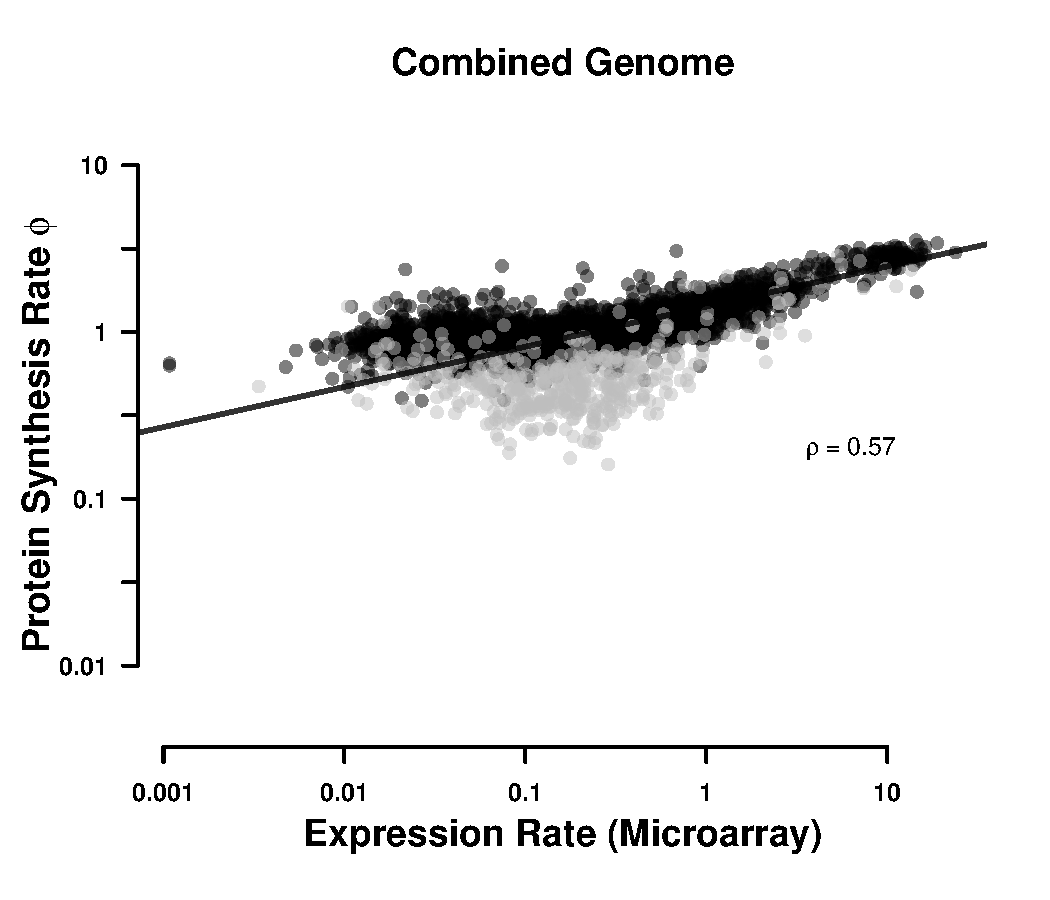
\includegraphics[width=.45\textwidth]{img/phi_corr_plot_whole_Genome_estim.pdf}
    \end{subfigure}
    \begin{subfigure}
        \centering
        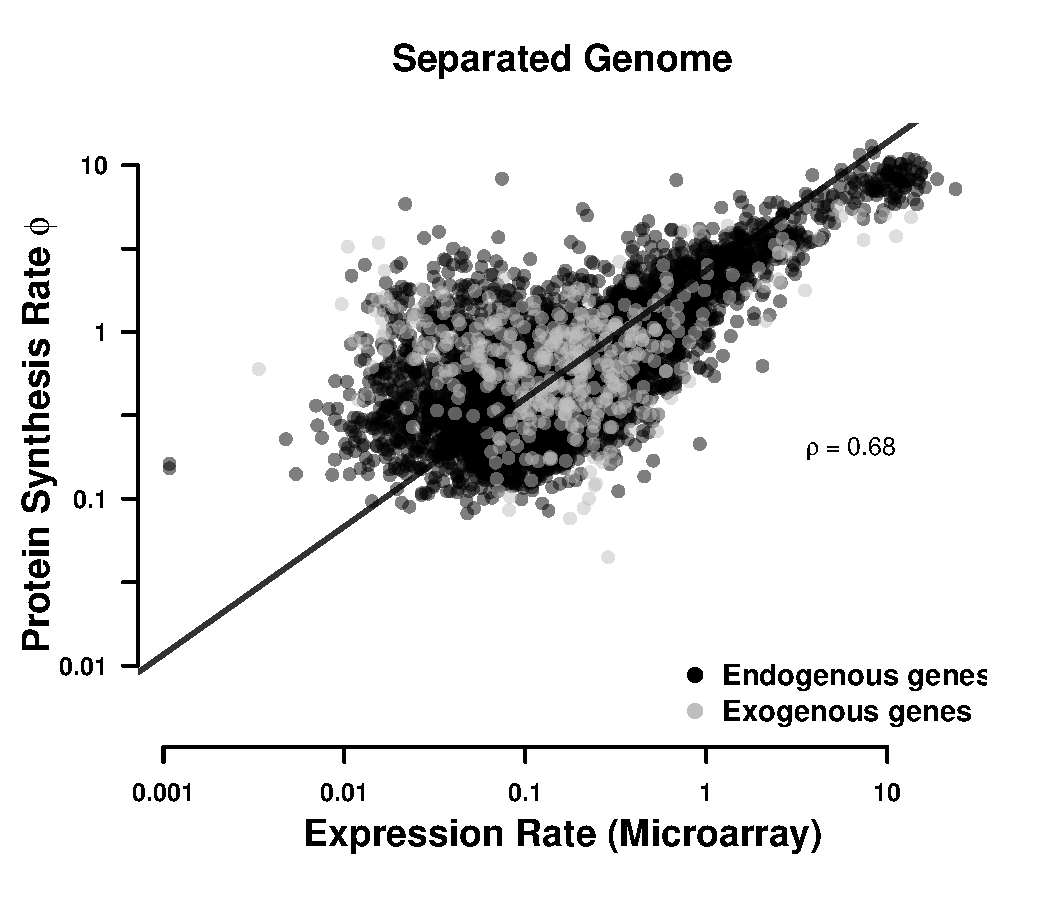
\includegraphics[width=.45\textwidth]{img/phi_corr_plot_split_Genome_estim.pdf}
    \end{subfigure}
    \caption{Put $\rho$ in plots, do I want two regression lines in plot? Only reporting overall regression so far. check if it is typeII regression}
    \label{fig:phi_corr_two_cond}
\end{figure}

In addition to model selection, we utilized independent information on gene expression to evaluate model fit.
Recognizing differences in \DM and \DE for the endogenous and exogenous gene sets substantially improves our ability to predict protein synthesis rate $\phi$ ($\rho = 0.69$ vs. $\rho = 0.59$ for the full genome;  Figure \ref{fig:phi_corr_two_cond}a,b).

\subsection*{Differences in the Endogenous and Exogenous Codon Usage}

Model selection and validation confirmed that the \kluyveri genome contains signatures of at least two cellular environments.
We compared the quantitative estimates of mutation bias (\DM) and selection bias (\DE) obtained from fitting \ROC to the endogenous and exogenous gene sets.
We find larger differences between \DM than \DE (Figure \ref{fig:csp_comp}). 
Estimates of \DM in the endogenous genes negatively correlate with the exogenous genes ($\rho = -0.49$) indicating strong differences in the mutation environment between \kluyveri and the donor lineage of the exogenous genes.
For example, $\sim 95 \%$ of codon families show mutation preference for A/T ending codons while, in contrast, the exogenous genes display an equally strong mutation bias towards C/G ending codons ($\sim 95 \%$).
Only the two codon amino acid Phenylalanine (Phe, F) shows complete concordance between endogenous and exogenous genes in mutation bias.
\begin{figure}[h]
    \centering
    \begin{subfigure}
        \centering
        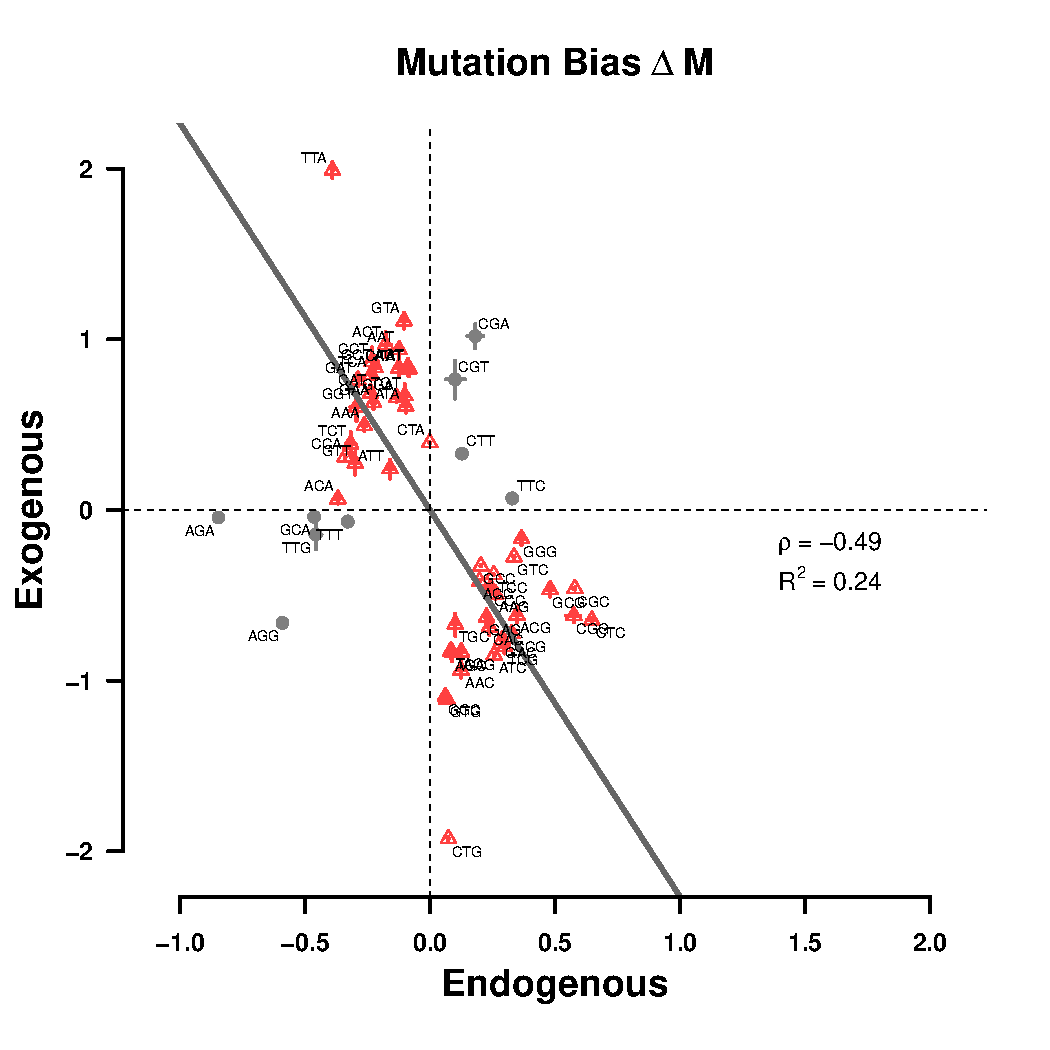
\includegraphics[width=.45\textwidth]{img/csp_corr_dm.pdf}
    \end{subfigure}
    \begin{subfigure}
        \centering
        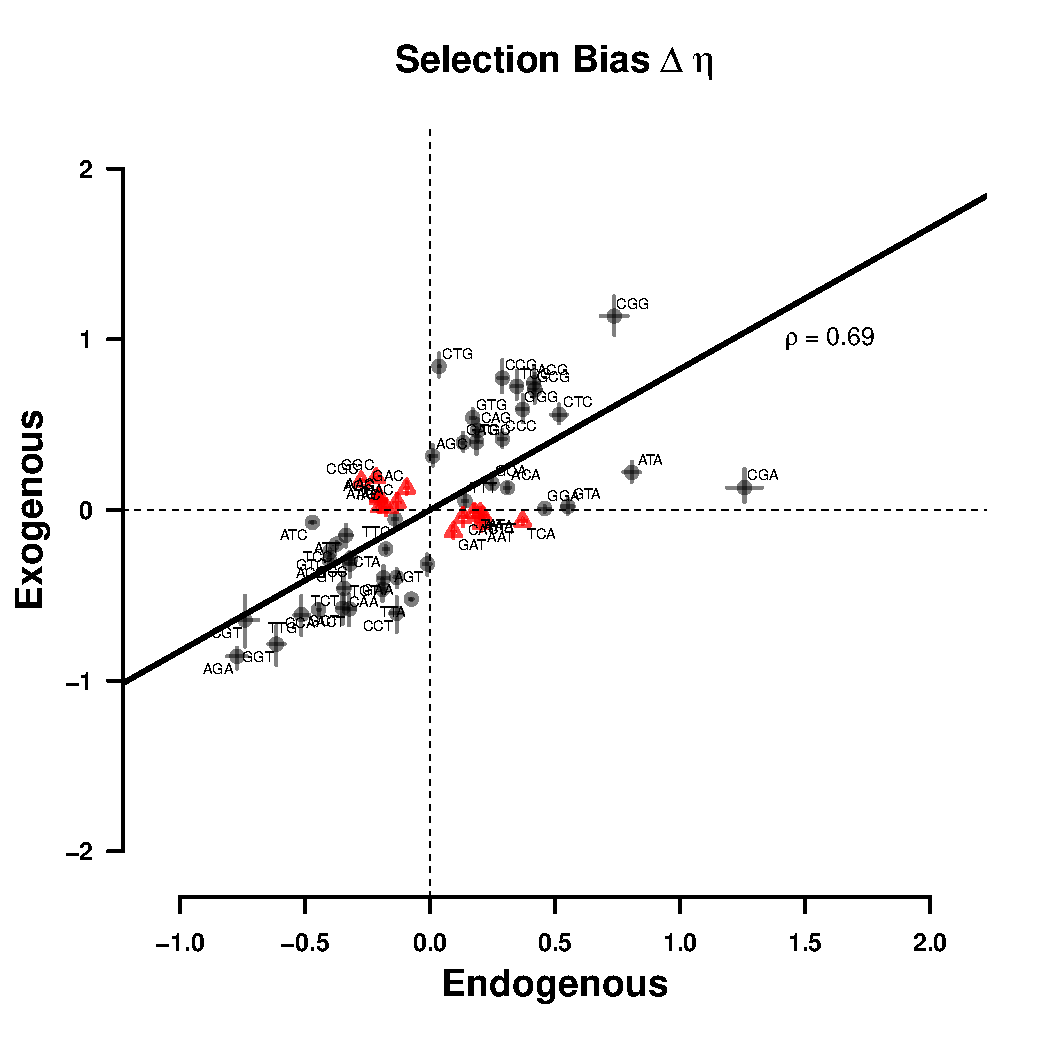
\includegraphics[width=.45\textwidth]{img/csp_corr_deta.pdf}
    \end{subfigure}
    \caption{Parameters are relative to mean ($R^2$ doesn't make sense, change to $\rho$, check $\Delta M$ regression line, looks off), check if it is typeII regression; rename to selection bias}
    \label{fig:csp_comp}
\end{figure}

Estimates of \DE show higher agreement between endogenous and exogenous genes ($\rho = 0.69$) than our estimates of \DM.
For nine amino acids selection favors the same codon in endogenous and exogenous genes.
Unlike the mutation bias, we find selection to be heavily biased towards A/T ending codons ($\sim 89 \%$) in the exogenous genes.
However, the selection environment in the endogenous genes is G/C biased ($\sim 58 \%$).
Thus, recognizing and treating endogenous and exogenous genes as separate sets avoids the inference of incorrect synonymous codon preferences (Table \ref{tab:codon_pref_deta}).

\subsection*{Determining Source of Exogenous Genes}

We combined our estimates of mutation bias ($\Delta M$) and selection bias ($\Delta \eta$) with synteny information and searched for potential source lineages of the introgressed region.
Of the 38 examinded yeast lineages only two ((\textit{Eremothecium gossypii} and \textit{Candida dubliniensis}) showed a strong positive correlation in codon usage (Figure \ref{fig:csp_endo_exo_comp}b).
\begin{figure}[h]
    \centering
    \begin{subfigure}
        \centering
        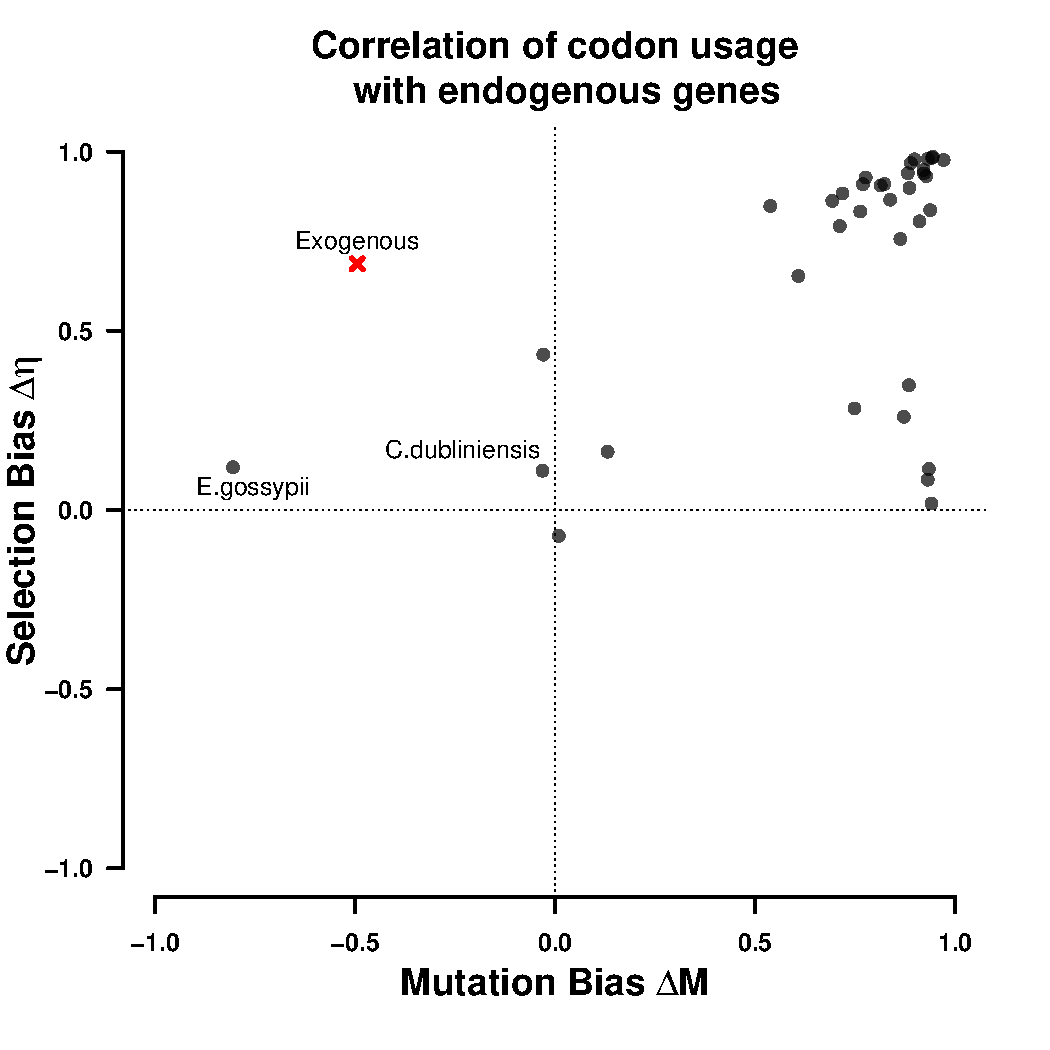
\includegraphics[width=.45\textwidth]{img/csp_mean_correlation_endo.pdf}
    \end{subfigure}
    \begin{subfigure}
        \centering
        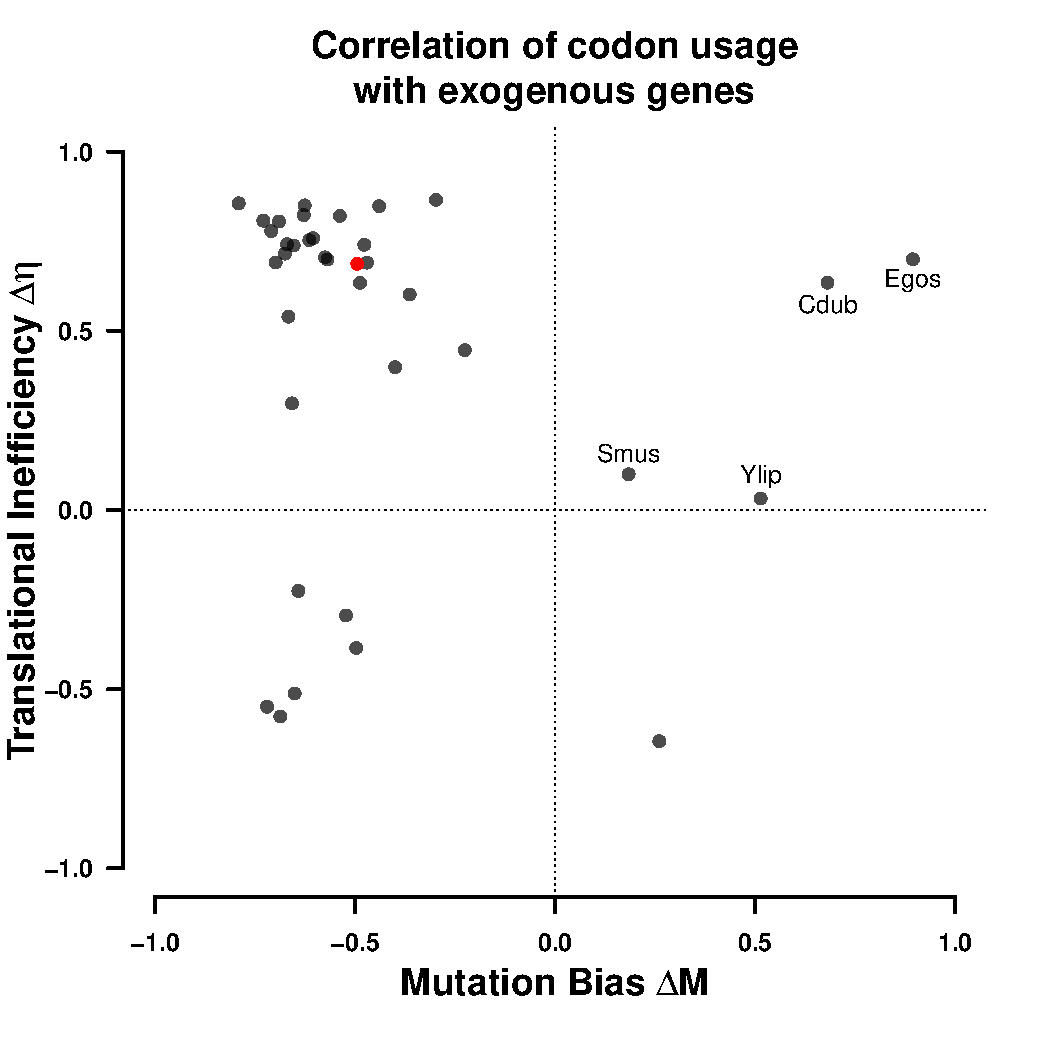
\includegraphics[width=.45\textwidth]{img/csp_mean_correlation_exo.pdf}
    \end{subfigure}
    \caption{check if it is typeII regression}
    \label{fig:csp_endo_exo_comp}
\end{figure}
The endogenous \kluyveri genome exhibits codon usage very similar to most yeast lineages examined, indicating little variation in codon usage among the examined yeasts (Figure \ref{fig:csp_endo_exo_comp}a).
The four lineages showing a positive $\Delta M$ and $\Delta \eta$ correlation with the exogenous genes have a weak to moderate positive correlation in selection bias with the endogenous genes; but, like the exogenous genes, tend to have a negative correlation in $\Delta M$ with the endogenous genes.

We compared synteny between the exogenous left arm of chromosome C and \gossypii and \dubl as well as closely related yeast species using SyMAP \citep{soderlund2006, soderlund2011}.
We find that \gossypii has the highest synteny coverage of all examined lineages, covering nearly the whole exogenous region (Figure \ref{fig:synteny_species}a)
In contrast, \dubl does not have a synteny relationship with the exogenous region.
Furthermore, the synteny relationship between the exogenous region and other yeasts appears to be limited to the Saccharomycetacease group(Figure \ref{fig:synteny_species}b).
Given these results, we conclude that the \gossypii lineage is the most likely source of the introgressed exogenous genes.

\subsection*{Estimating Introgression Age}

We estimated the introgression age using an exponential model of decay of mutation bias assuming that \gossypii with its current mutation bias is still representative of the mutation bias in the source lineage.
We utilize the \DM estimates for all two codon amino acids and infered the age of the introgression to be on the order of $6\times 10^8 \pm X\times 10^8$ generations. 
We assume a mutation rate of $3.8\times 10^{-10}$ per nucleotide per generation, a value in line with other estimates \citep{zhu2014, lang2008}.
\kluyveri experiences between one and eight generations per day, we therefore expect the introgression to have occurred about 205,000-1,600,000 years ago, longer than previous estimates \citep{friedrich2015}.
However, our estimates are likely overestimates as they assume a purely neutral decay.

Furthermore, we estimated the persistence of the foreign genomic environment.
Assuming that differences in mutation bias will decay more slowly than differences in selection bias, we predict that the foreign genomic environment will have decayed to one percent of the \kluyveri environment within about $5\times 10^9$ generations.


\subsection*{Fitness Burden of the Exogenous Genes}

Estimates of selection bias for the exogenous genes show that, while well correlated with the endogenous genes, only nine amino acids have the same codon preference.
We therefore expect that the introgressed genes represent a significant reduction in fitness for \kluyveri, and even more so at the time of introgression.
As the introgression occurred before the diversification of \kluyveri and has fixed since then throughout the various populations, we are left without the original chromosome arm \citep{friedrich2015}.
However, using our estimates of $\Delta M$ and $\Delta \eta$ from the endogenous genes, we can estimate the fitness burden of the exogenous genes relative to an expected gene set.
\begin{figure}[h]
    \centering
    \begin{subfigure}
        \centering
        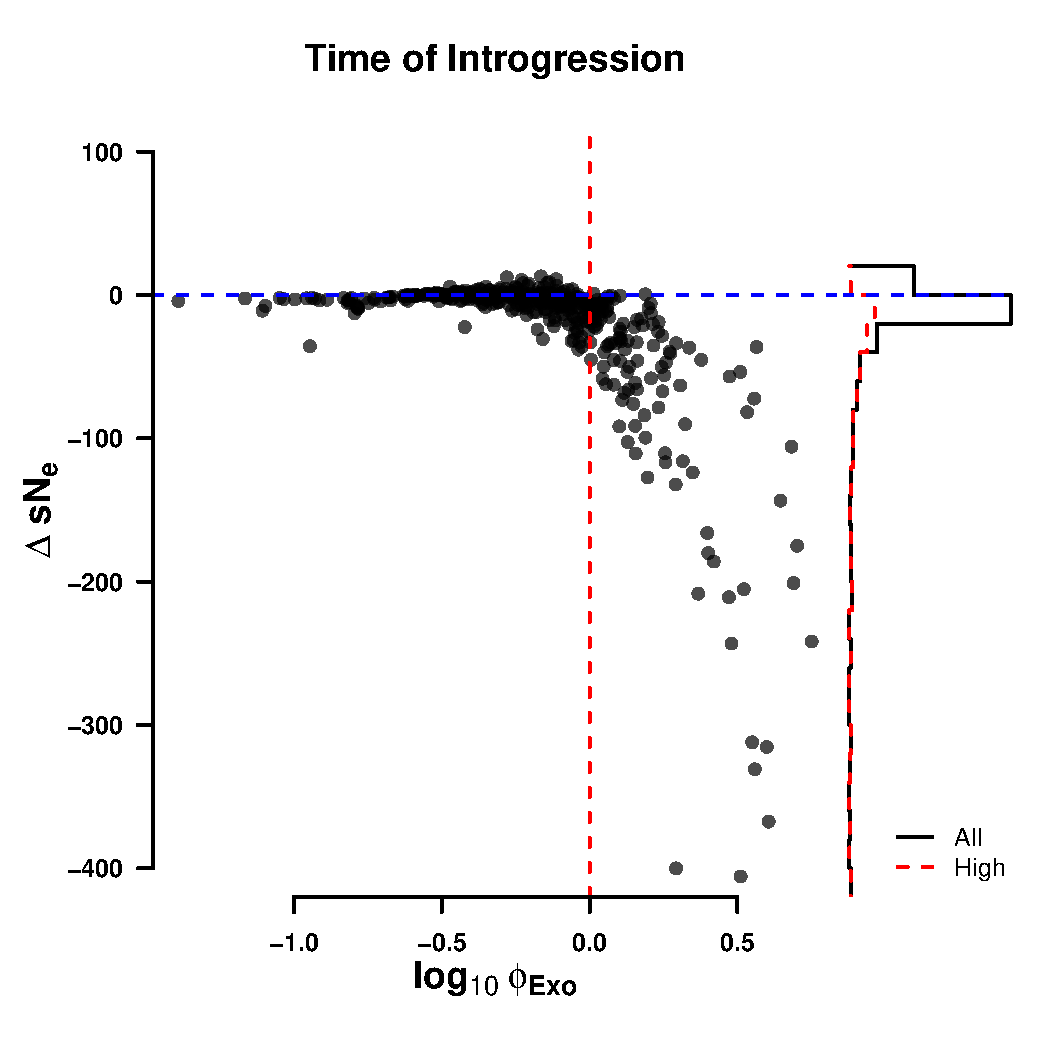
\includegraphics[width=.45\textwidth]{img/fitness_difference_gos_kappa5.pdf}
    \end{subfigure}
    \begin{subfigure}
        \centering
        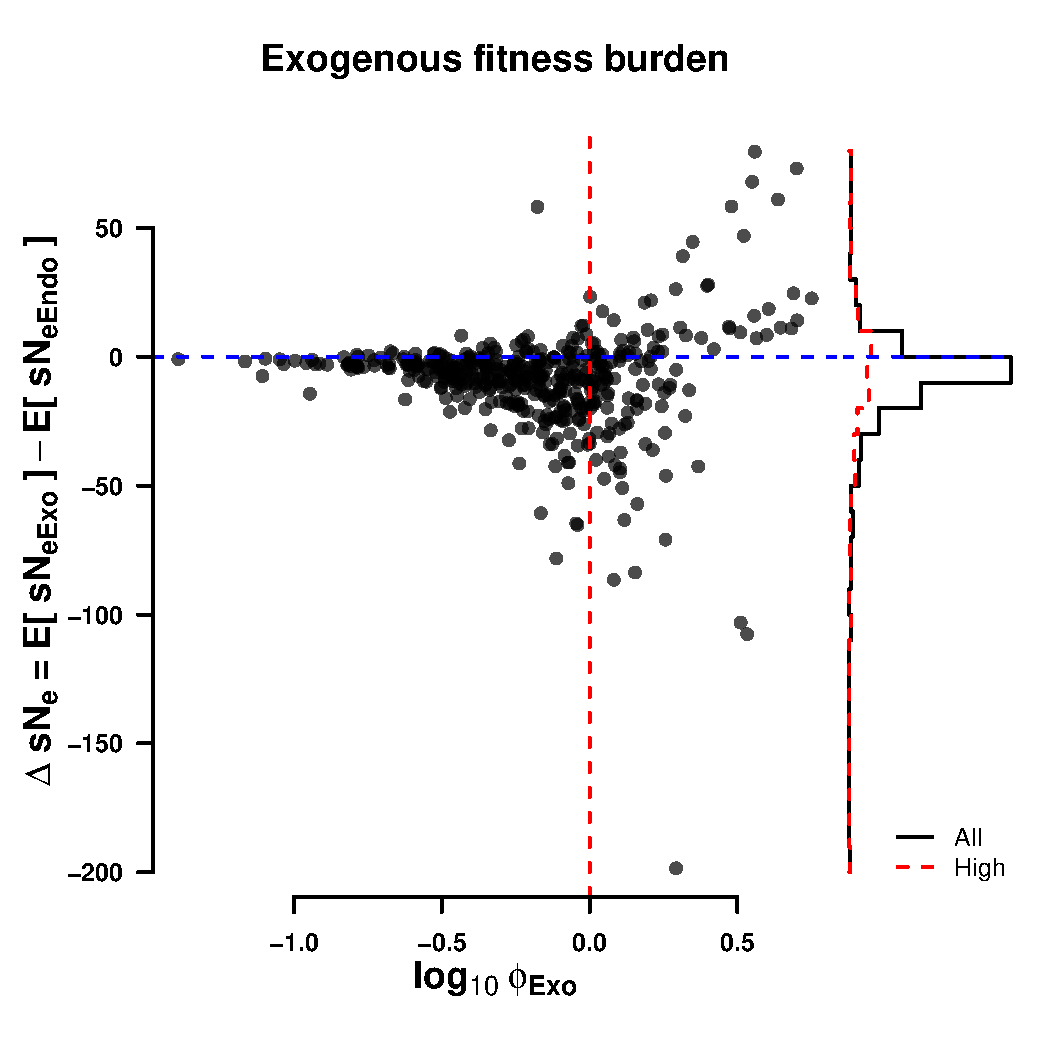
\includegraphics[width=.45\textwidth]{img/fitness_difference_exo.pdf}
    \end{subfigure}
    \caption{Fitness burden at time of introgression (left) using scaled $\phi$, and currently (right). Simplify y-axis label, put in description}
    \label{fig:sne_fitness_burden}
\end{figure}

We estimate the genetic load of the exogenous genes at the time of introgression (Figure \ref{fig:sne_fitness_burden}a) and currently (Figure \ref{fig:sne_fitness_burden}b).
These estimates are dependent on three key assumptions.
First, we assume again that the current genomic environment of \gossypii is reflective of the ancestral environment.
Second, we assume that the current amino acid composition of the exogenous genes is the same as in the replaced endogenous genes.
Third, we assume that the difference in the efficacy of selection between \gossypii and \kluyveri can be described with a simple scaling term on protein synthesis rate $\phi$ (Figure \ref{fig:sne_scaling}b).

At the time of the introgression, only a few genes were weakly exapted (Figure \ref{fig:sne_fitness_burden}a) with all high expression genes ($\phi > 1$) being mal-adapted to the novel cellular environment.
However, these highly expressed genes show the greatest level of adaptationto the \kluyveri cellular genomic environment (Figures \ref{fig:sne_fitness_burden}a, \ref{fig:adapt_tot}).

\section*{Discussion}

We show that the \kluyveri genome contains two distinct signatures of cellular environments, its own endogenous and a foreign exogenous one obtained by an introgression event.
Following \citet{payen2009}, who defined the boundary of the anomalous chromosome region based on its elevated \GC, we partitioned the \kluyveri genome into an endogenous and an exogenous gene set using gene location.
We estimated the codon usage of the entire \kluyveri genome and the separated endogenous and exogenous gene sets (Figure \ref{fig:cub_all_sets}).
Both, Mutation bias and selection bias differ between endogenous and exogenous genes.
The endogenous genes show a strong mutation bias towards A/T ending codons, however, mutation is biases towards G/C ending codons in the exogenous genes.
This tendency is reversed in selection bias, leading to a strong mismatch in codon usage between the gene sets, supporting our notion of two distinct signatures of codon usage.

Only nine codon families share the same optimal codon in the endogenous and egogenous gene sets.
Nevertheless, we find that in both gene sets mostly the same codons are selected for, indicated by the high correlation of \DE estimates between the two gene sets.
However, the strength of selection within a codon family differes between gene sets, causing a change in rank order.
Exceptions are e.g. XXX where XXX is favored by selection in the endogenous genes while XXX is favored in the exogenous genes.
Out of the nine synonymous codon families with differing codon preferences, the entire \kluyveri genome appears to share the exogenous codon preference seven times (Table \ref{tab:codon_pref_deta}).
We find even greater discordance in our estimates of \DM (Table \ref{tab:codon_pref_dm}).
Without recognizing this difference in codon preference our estimates would not have been reflective of the actual codon usage of the \kluyveri genome but of a relatively small introgressed gene set.
This shows that a small number of exogenous genes ($\sim 9 \%$ of genes) can have a disproportional impact on our estimates of \DM and \DE when fitting \ROC to the entire \kluyveri genome.
While this is surprising, it further highlights the importance to recognize differences in codon usage within a genome.
These results also indicate that we can attribute the higher \GC in the exogenous genes mostly to differences in mutation bias favoring G/C ending codons.

Separating the endogenous and exogenous genes improves our estimates of protein synthesis rate $\phi$ by $17 \%$ relative to the full genome estimate.
Furthermore, we find that the variation in our estimates of $\phi$ is more consitent with the current understanding of gene expression (compare Figure \ref{fig:phi_corr_two_cond}a and b). 
Small variation in $\phi$ estimates may serve as an indicator for the presents of multiple genomic environments in future work.
In the case of the \kluyveri genome, finding a severe mismatch in \DM causes $\phi$ values for low expression genes ($\phi < 1$) to increase towards the inflection point where the dominance of mutation gives way to selection.
In the case of the two codon amino aicds, the inflection point represents the point at which mutation and selection are contributing equally to the probability of a codons occurence.
We find this inflection point around $\phi = 1$ for most amino acids (Figure \ref{fig:cub_all_sets}). 
However, \ROC assumes that estimates of $\phi$ follow a log-normal distribution with an expected value $E[\phi] = 1$ allowing us to interpret \DE as the average strength of selection relative to drift ($\overline{sNe}$) for the average gene, but also tying the mean and standard deviation of the prior distribution together.
Therefore, an increase in $\phi$ for low expression genes has to be meet with a decrease of $\phi$ for high expression genes, reducing the overall variance in $\phi$ ; see \citet{gilchrist2015} for details. 

Having shown that the introgressed exogenous genes reflect a foreign genomic environment, we used the quantitative estimates of \DM and \DE from \ROC to identify potential source lineages.
The comparison of the endogenous and exogenous \DM and \DE estimates to 38 other yeast lineages revealed that most yeasts examined share similarity in mutation bias (Figure \ref{fig:csp_comp}ab).
Similar, we find strong similarities in selection bias between examined yeasts, potentially indicating stabilizing selection on codon usage.
However, the exogenous genes do not share this commonality (Figure \ref{fig:csp_comp}a), as their mutation bias strongly deviates from the endogenous genes and most other yeast species examined. 
This large difference in mutation bias between endogenous and exogenous genes allowed us to limit our candidate list to only two likely lineages, \dubl and \gossypii.
Interestingly, we did not find \textit{Lachancea thermotolerance}, a thermophilic lineage closely related to \kluyveri, as a potential candidate.
While \textit{L. thermotolerance} does have a strong synteny relationship with \kluyveri, it does not show similarity in codon usage with the exogenous genes and does not share their high \GC.

Inference of synteny relationships between the exogenous region and \dubl and \gossypii as well as closely related species showed that synteny relationship is limited to the Saccharomycetaceae clade (Figure \ref{fig:synteny_species}b).
\gossypii showed the highest syntenty coverage and is the only species with similar codon usage.
Furthermore, \gossypii is the only species examined with a \GC $> 50 \%$ like it is observed in the exogenous region.
The synteny coverage extends along the whole exogenous regions with the exception to the very 3' and 5' end of the region. 
The lack of coverage at the ends of the region also coincides with a drop in \GC, potentially indicating remains of the original replaced region or increased adaptation.
The ancestral introgressed region may have also broken up in \gossypii as we find non overlapping synteny with chromosomes $VI$ and $V$ as well as have indication that the C chromosome of \kluyveri very robust to recombination events \citep{payen2009, vakirlis2016}. 

With \gossypii identified as potential source lineage of the introgressed region, we inferred the time past since the introgression occurred using our estimates of mutation bias \DM.
The \DM estimates are well suited for this task as they are free of the influence of selection and unbiased by $N_e$ and other scaling terms, which is in contrast to our estimates of \DE \citep{gilchrist2015}.
We estimated the time since introgression to be on the order of $6\times 10^8$ generations, which is a much longer time than a previous estimate by \citet{friedrich2015} of a minimum of $55.5\times 10^6$ generations .
However, it must be highlighted that our estimate implicitly assumes neutrality and is therefore a conservative estimate, potentially overestimating the time since introgression. 
Our estimate also depend on the assumption that the \gossypii genomic environment reflects the ancestral environment at the time of the introgression.
If the the ancestral mutation environment was more similar to the \kluyveri environment at the time of the introgression than the \gossypii environment is today, we would overestimate this time.
On the other hand, we would underestimate the time since introgression if the two genomic environments were more dissimilar.

The estimates of mutation bias \DM also allow us the infer the time until the signature of the foreign genomic environment will have decayed.
Our estimate of decay is an order of magnitude greater than our estimate of the time since introgression ($5\times 10^9$ and $6\times 10^8$ generations).
Estimates of decay based on \DM are more conservative as we expect differences in \DE to decay before due to selection favoring the decay.
 
As we have determined that the introgression event has a long persisting foreign signature, it is important to understand the fitness consequences of such an event.
In particular as it is an open question how codon usage changes.
It is however, assumed that a selection has to favor shift in codon usage over a long period of time \citep{Hershberg2008}, a situation clearly present in the \kluyveri genome.
We estimated the reduction in fitness that the exogenous genes represent assuming that the replaced endogenous genes and the new exogenous genes had a common amino acid composition.
This assumption, along with the assumption that the current \kluyveri cellular environment is reflective of the cellular environment at the time of the introgression is necessary to estimate the expected endogenous sequence that was replaced.
Our results show that individual low expression genes contribute little to the fitness cost, and show less adaptation to the novel cellular environment (Figure \ref{fig:sne_fitness_burden}a,b, \ref{fig:adapt_tot}).
A small number of low expression genes even appear exapted likely due to the mutation bias in the endogenous genes matching the selection bias in the exogenous genes, as both are G/C biased. 
Highly expressed genes on the other hand have greatly adapted to the \kluyveri cellular environment.
This, however does not mean that these genes show a higher rate of evolution but that small changes in their sequence have large impacts on the fitness burden these sequences represent.
In fact we have no evidence that the exogenous genes evolve faster than their endogenous counterparts.
This is consistent with the wide body of work showing overall rates of change for high expression genes tend to be slower than in low expression genes.
To this day, the exogenous genes represent a significant fitness burden on \kluyveri.
\marginpar{Trying to think about it having reached fixation, there is no alternative cleft in the population to compete with.}
However, as the introgression appears to have reached fixation \citep{friedrich2015}, the fitness burden relative to the replaced chromosome arm is only of theoretical interest.

The high fitness burden the exogenous genes represented at the time of the introgression indicates that the introgression was a very unlikely event to have reached fixation in a population with a large $N_e$ as it is typical for yeasts.
It is hard to contextualize the probability of this introgression going to fixation as we are not aware of any estimates of the frequency at which such large scale introgressions of genes with very different signatures of codon usage occur.
However, \kluyveri diverged about 85 Mya ago from the rest of the Lachancea clade.
This represents between $10^{10}$ to $10^{11}$ generations.
Assuming a for yeasts typical effective population size on the order of $10^8$, we are left with $10^{18}$ to $10^{19}$ opportunities for such an event to occur.
In addition, the strong mutation bias towards G/C ending codons in the exogenous genes may have contributed to the fixation of this introgression (include figure of \DM v \DE).
It is, on the other hand, also possible that the exogenous genes have represented a fitness increase due to external envrionemntal factors decpide their mismatch in codon usage; resulting in the fixation of the introgression.
 
In conclusion, our results show the usefulness of the separation of mutation bias and selection bias and the importance of recognizing the presents of multiple genomic environments in the study of codon usage.
We also illustrate how a mechanistic model like \ROC and the quantitative estimates it provides can be used for more sophisticated hypothesis testing in the future.
In contrast to other approaches used to study codon usage like CAI \citep{sharp1987} or tAI \citep{dosreis2004}, \ROC is not agnostic to differences in mutation bias.
We highlight potential pitfalls when estimating codon preferences, as estimates can be biased by the signature of a second, historical genomic environment.
In addition, we show how quantitative estimates of mutation bias and selection relative to drift can be obtained from codon data and used to infer the fitness cost of an introgression as well as its history and potential future.


\section*{Materials and Methods}

\subsection*{Separating endogenous and exogenous genes}
A GC-rich region was identified by \citet{payen2009} in the \kluyveri genome extending from position 1 to 989,693 of chromosome C.
This region was later identified as an introgression by \citet{friedrich2015}.
We obtained the \kluyveri genome from SGD Project \url{http://www.yeastgenome.org/download-data/} (last accessed: XX-XX-XXXX) and the annoation for \kluyveri NRRL Y-12651 (assenbly ASM14922v1) from NCBI (last accessed: XX-XX-XXXX).
We assigned XXX genes located on chromosome C with a location within the $\sim 1 Mb$ window to the exogenous gene set.
All other XXX genes of the \kluyveri genome were assigned to the exogenous genes.
All genes could be uniquly assigned to one or the other gene set.

\subsection*{Fitting \ROC}
We used AnaCoDa \citep{landerer2018}.

\subsection*{Comparing codon specific parameter estimates}

\subsection*{Synteny}

\subsection*{Determining introgression timeline}
ODE system solved with Mathematica

\subsection*{Estimating fitness burden}


\section*{Acknowledgments}

This work was supported in part by NSF Awards MCB-1120370 (MAG and RZ) and DEB-1355033 (BCO, MAG, and RZ) with additional support from The University of Tennessee Knoxville. 
CL received support as a Graduate Student Fellow at the National Institute for Mathematical and Biological Synthesis, an Institute sponsored by the National Science Foundation through NSF Award DBI-1300426, with additional support from UTK. 
The authors would like to thank Brian C. O'Meara and Alexander Cope for their helpful criticisms and suggestions for this work.


\bibliographystyle{unsrtnat}
\bibliography{kluyveri_paper}

\clearpage
\section*{Supplementary Material}
\beginsupplement

Supporting Materials for \emph{Fitness consequences of mismatched codon usage} \ by Landerer \emph{et al.}.


\begin{table}
    \centering
\begin{tabular}{  l  c  c  c  c  }
\hline
	Amino Acid & \gossypii & Endogenous & Exogenous & \kluyveri \\ \hline \hline
	Ala A & GCG & GCA & GCG & GCG \\ \hline
	Cys C & TGC & TGT & TGC & TGC \\ \hline
	Asp D & GAC & GAT & GAC & GAC \\ \hline
	Glu E & GAG & GAA & GAG & GAG \\ \hline
	Phe F & TTC & TTT & TTT & TTT \\ \hline
	Gly G & GGC & GGT & GGC & GGC \\ \hline
	His H & CAC & CAT & CAC & CAC \\ \hline
	Ile I & ATC & ATT & ATC & ATA \\ \hline
	Lys K & AAG & AAA & AAG & AAA \\ \hline
	Leu L & CTG & TTG & CTG & CTG \\ \hline
	Asn N & AAC & AAT & AAC & AAT \\ \hline
	Pro P & CCG & CCA & CCG & CCG \\ \hline
	Gln Q & CAG & CAA & CAG & CAG \\ \hline
	Arg R & CGC & AGA & AGG & CGG \\ \hline
	Ser$_4$ S & TCG & TCT & TCG & TCG \\ \hline
	Thr T & ACG & ACA & ACG & ACG \\ \hline
	Val V & GTG & GTT & GTG & GTG \\ \hline
	Tyr Y & TAC & TAT & TAC & TAC \\ \hline
	Ser$_2$ Z & AGC & AGT & AGC & AGC \\ \hline
\end{tabular}
    \caption{Synonymous codon preference in the various data sets based on our estimates of $\Delta M$}
    \label{tab:codon_pref_dm}
\end{table}

\clearpage

\begin{table}
    \centering
\begin{tabular}{  l  c  c  c  c  }
\hline
	Amino Acid & \gossypii & Endogenous & Exogenous & \kluyveri \\ \hline \hline
	Ala A & GCT & GCT & GCT & GCT \\ \hline
	Cys C & TGT & TGT & TGT & TGT \\ \hline
	Asp D & GAT & GAC & GAT & GAT \\ \hline
	Glu E & GAA & GAA & GAA & GAA \\ \hline
	Phe F & TTT & TTC & TTC & TTC \\ \hline
	Gly G & GGA & GGT & GGT & GGT \\ \hline
	His H & CAT & CAC & CAT & CAT \\ \hline
	Ile I & ATA & ATC & ATT & ATT \\ \hline
	Lys K & AAA & AAG & AAA & AAG \\ \hline
	Leu L & TTA & TTG & TTG & TTG \\ \hline
	Asn N & AAT & AAC & AAT & AAC \\ \hline
	Pro P & CCA & CCA & CCT & CCA \\ \hline
	Gln Q & CAA & CAA & CAA & CAA \\ \hline
	Arg R & AGA & AGA & AGA & AGA \\ \hline
	Ser$_4$ S & TCA & TCC & TCT & TCT \\ \hline
	Thr T & ACT & ACC & ACT & ACT \\ \hline
	Val V & GTT & GTC & GTT & GTT \\ \hline
	Tyr Y & TAT & TAC & TAT & TAC \\ \hline
	Ser$_2$ Z & AGT & AGT & AGT & AGT \\ \hline
\end{tabular}
    \caption{Synonymous codon preference in the various data sets based on our estimates of $\Delta \eta$}
    \label{tab:codon_pref_deta}
\end{table}

\clearpage

\begin{figure}[h]
    \centering
    \begin{subfigure}
        \centering
        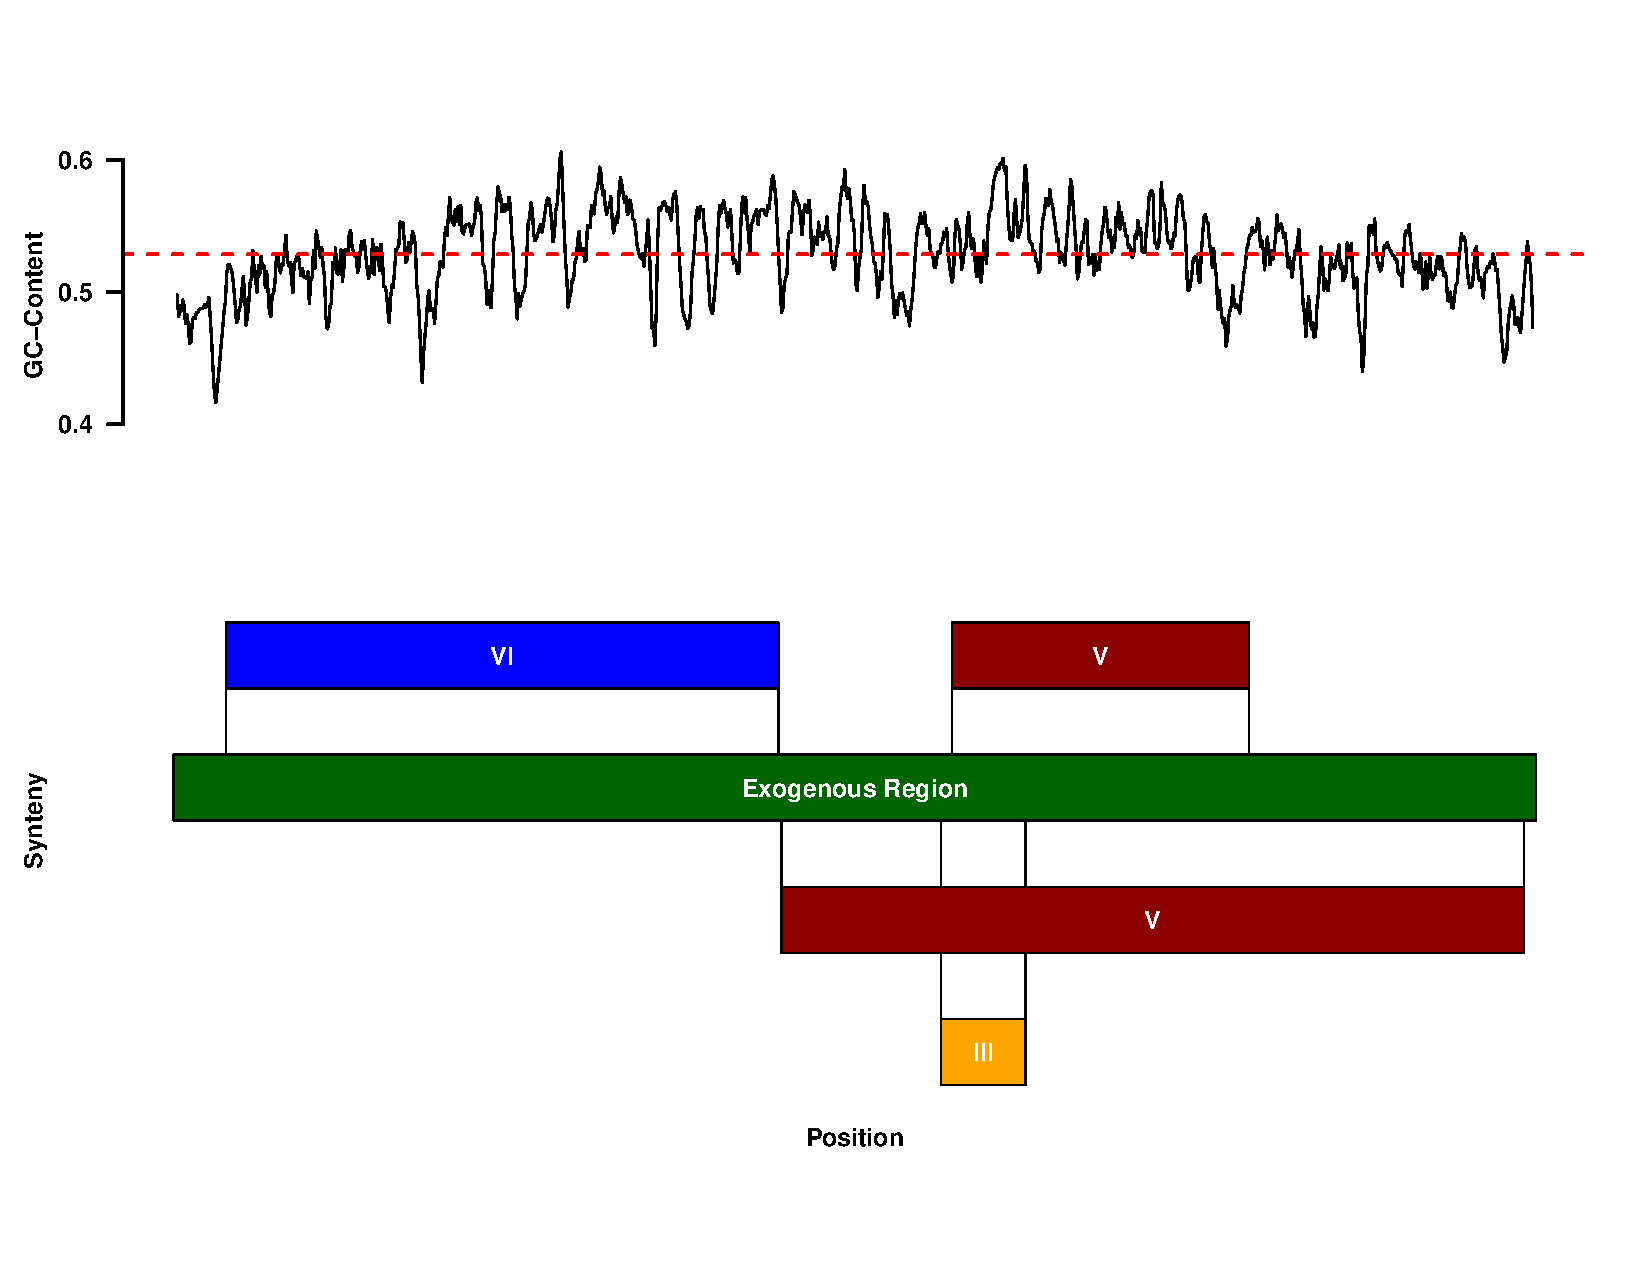
\includegraphics[width=.45\textwidth]{img/synteny_blocks_and_gc.pdf}
    \end{subfigure}
    \begin{subfigure}
        \centering
        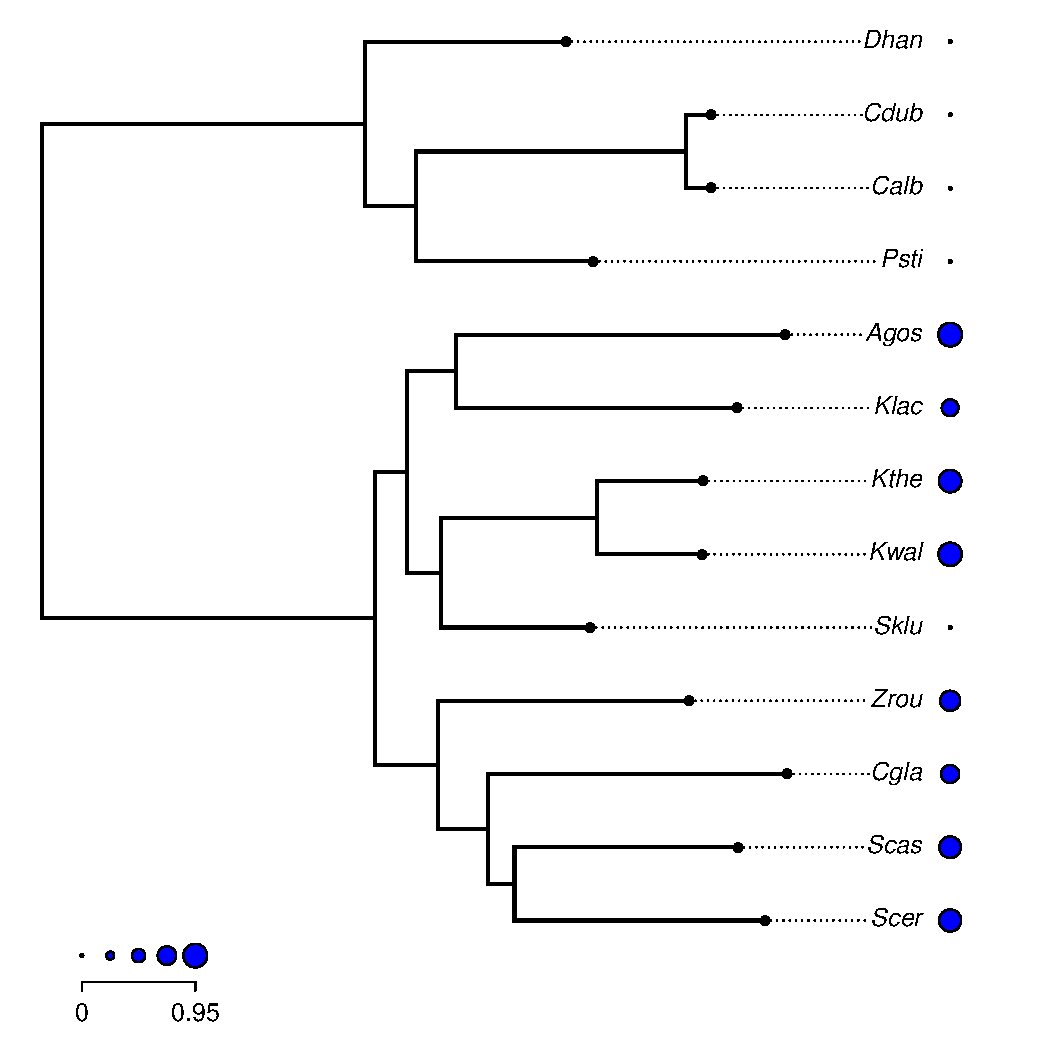
\includegraphics[width=.45\textwidth]{img/synteny_coverage.pdf}
    \end{subfigure}
    \caption{Suppl Fig: Synteny relationship of \gossypii and the exogenous genes (left), Amount of synteny for each species (Units of std dev) checked for synteny.}
    \label{fig:synteny_species}
\end{figure}

\begin{figure}[h]
    \centering
    \begin{subfigure}
        \centering
        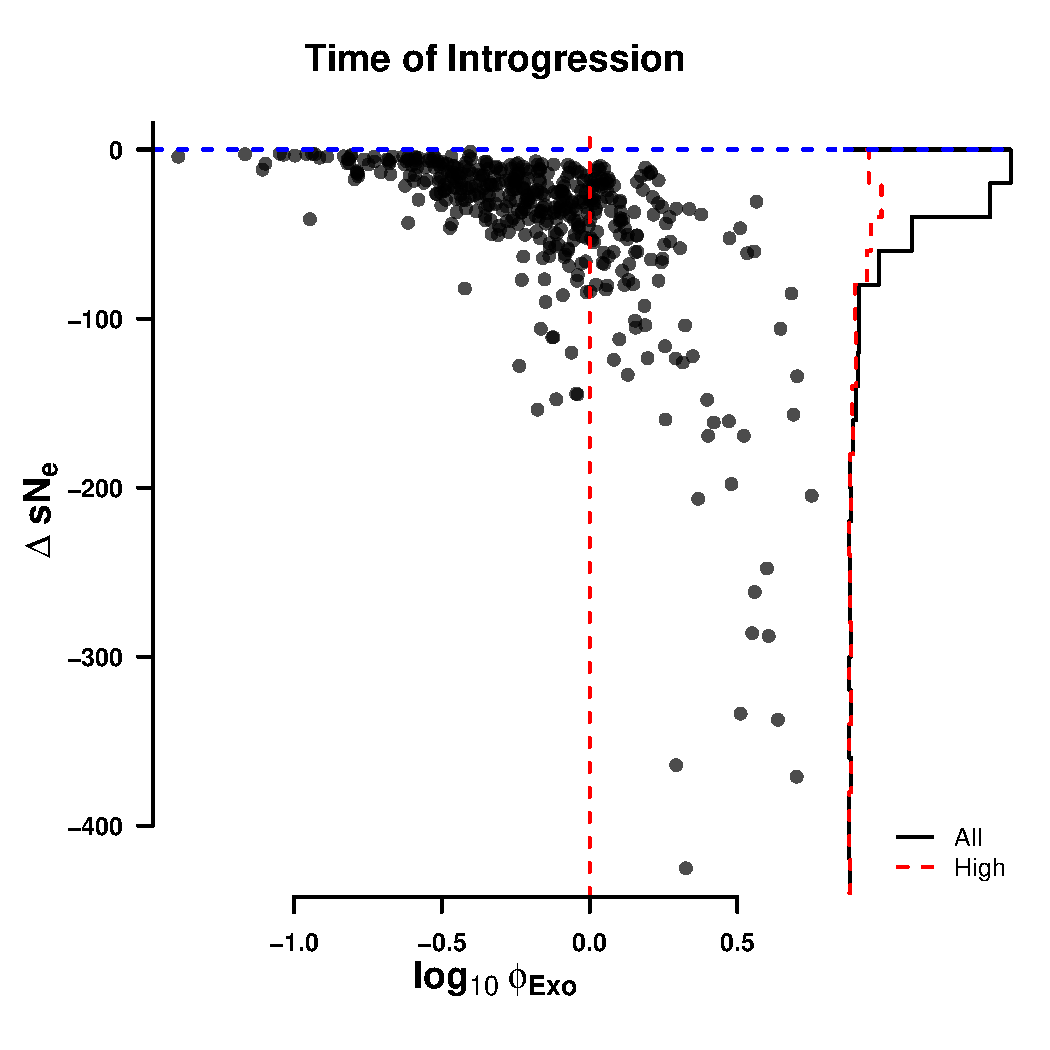
\includegraphics[width=.45\textwidth]{img/fitness_difference_gos_kappa1.pdf}
    \end{subfigure}
    \begin{subfigure}
        \centering
        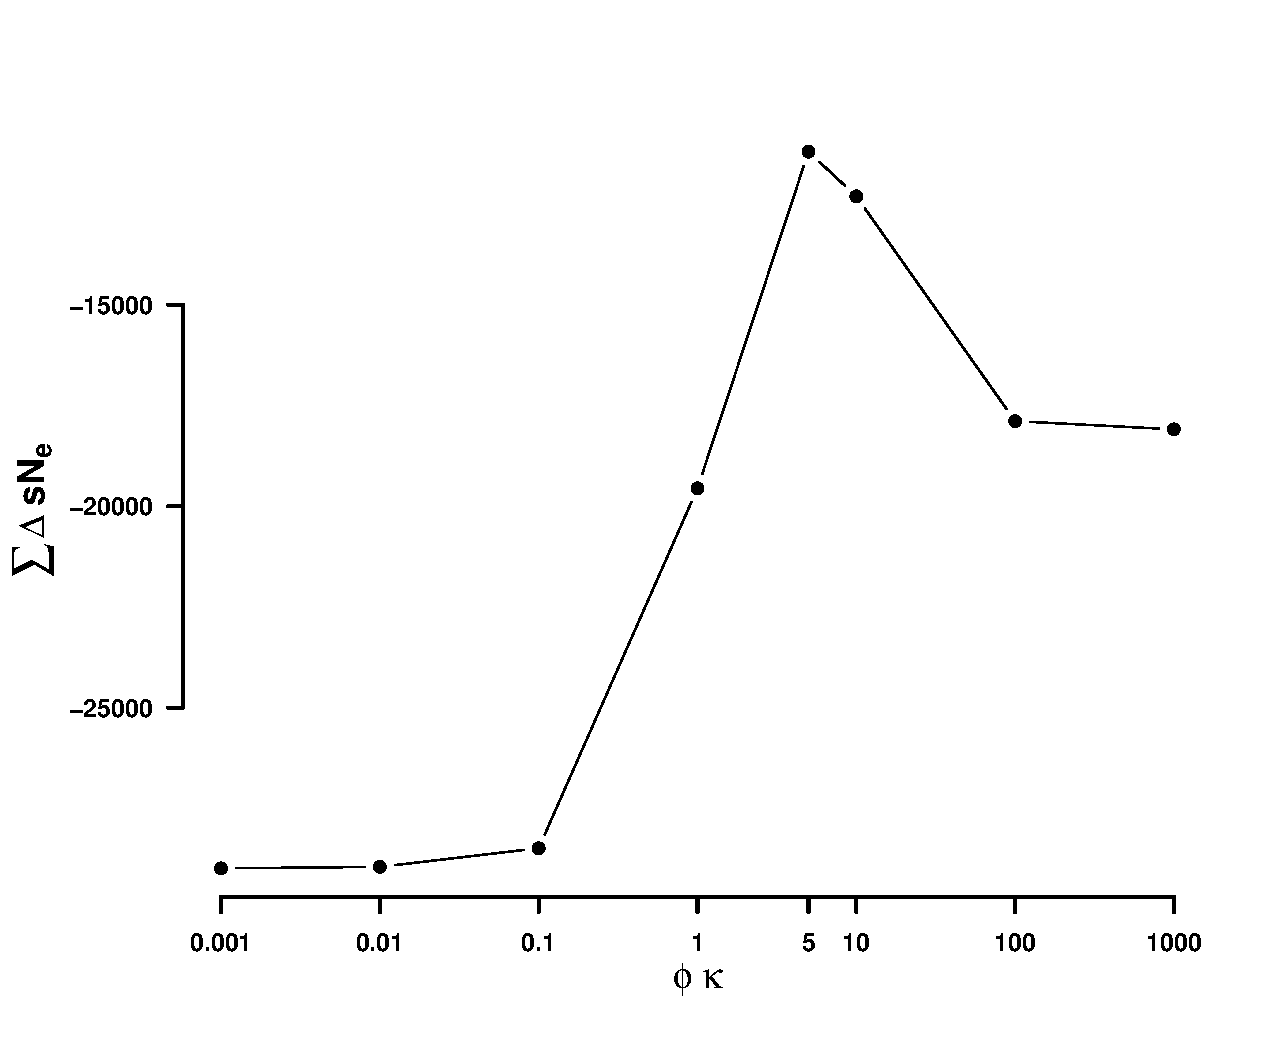
\includegraphics[width=.45\textwidth]{img/fitness_phi_scaling_gos.pdf}
    \end{subfigure}
    \caption{Suppl Fig: Fitness burden (left) without scaling of $\phi$, and change of total fitness burden with scaling $\kappa$}
    \label{fig:sne_scaling}
\end{figure}

\begin{figure}[H]
     \centering
	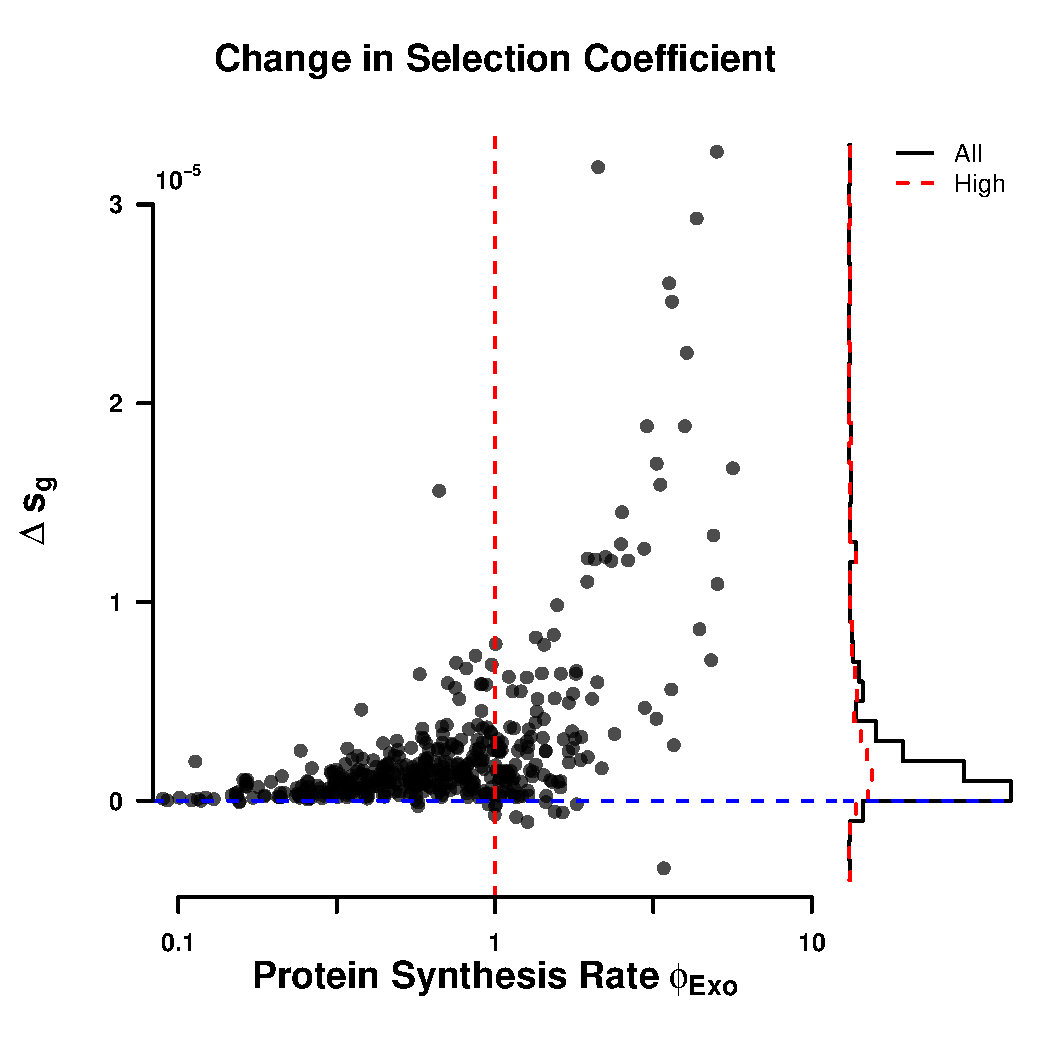
\includegraphics[width=\textwidth]{img/adaptation_total.pdf}
	\caption{Total amount of adaptation between time of introgression and now}
	\label{fig:adapt_tot}
\end{figure}

\clearpage
\begin{figure}[H]
     \centering
	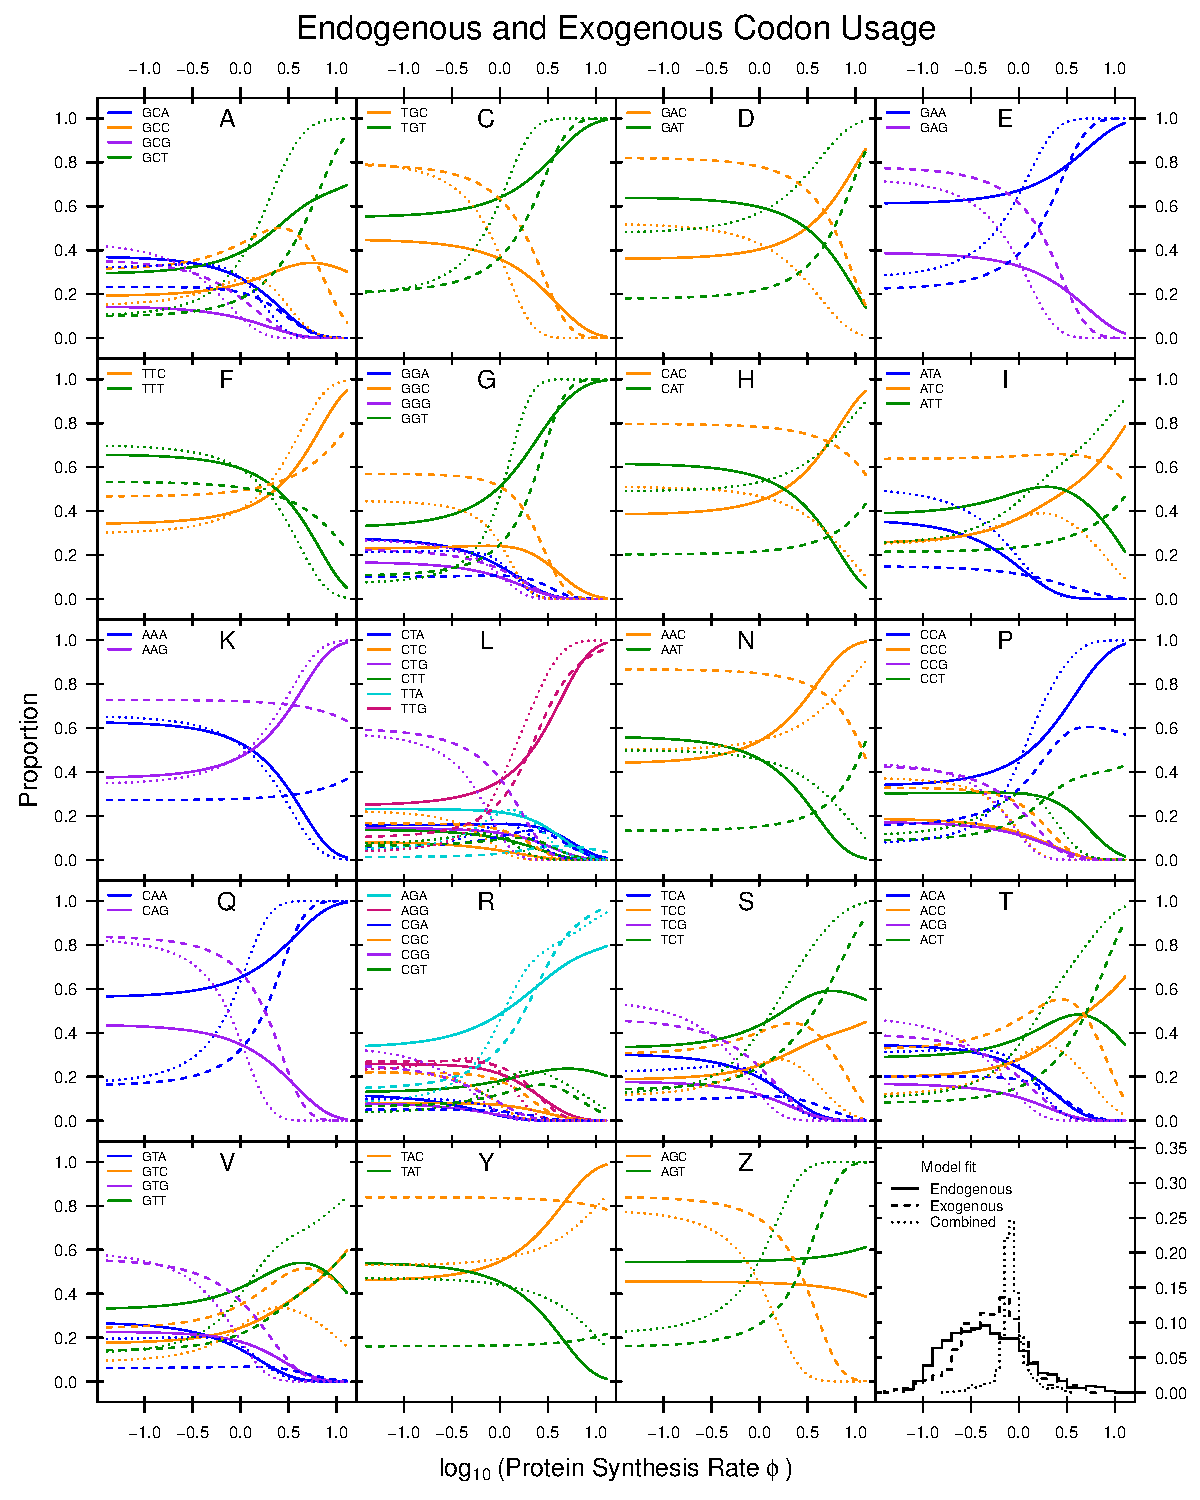
\includegraphics[width=\textwidth]{img/CUB_cleft_main.pdf}
	\caption{Suppl Fig}
	\label{fig:cub_all_sets}
\end{figure}

\end{document}
